\documentclass[a4paper,12pt,article]{memoir}
\usepackage{amsmath}
\usepackage{amssymb}
\usepackage{mathspec}
\usepackage{xltxtra}
\usepackage{polyglossia}
\usepackage{MnSymbol}
\usepackage{siunitx,cancel,graphicx}
\usepackage{enumitem}
\usepackage{hyperref,graphicx}
\usepackage{icomma}
\usepackage{float}
\usepackage{mleftright}

\usepackage{listings}
\usepackage{color}
\usepackage{xcolor}

\usepackage[
backend=biber,
style=numeric,
citestyle=numeric,
sorting=none
]{biblatex}
\addbibresource{resources.bib}


% This is the color used for MATLAB comments below
\definecolor{MyDarkGreen}{rgb}{0.0,0.4,0.0}
\definecolor{Blue}{rgb}{0.0,0.0,1.0}
\definecolor{Purple}{rgb}{1.0,0.0,1.0}

\colorlet{mygray}{black!30}
\colorlet{mygreen}{green!60!blue}
\colorlet{mymauve}{red!60!blue}

\lstset{
  backgroundcolor=\color{gray!10},
  basicstyle=\ttfamily,
  columns=fullflexible,
  breakatwhitespace=false,
  breaklines=true,
  captionpos=b,
  commentstyle=\color{mygreen},
  extendedchars=true,
  frame=single,
  keepspaces=true,
  keywordstyle=\color{blue},
  language=c++,
  numbers=none,
  numbersep=5pt,
  numberstyle=\tiny\color{blue},
  rulecolor=\color{mygray},
  showspaces=false,
  showtabs=false,
  stepnumber=5,
  stringstyle=\color{mymauve},
  tabsize=3,
  title=\lstname
}






\setdefaultlanguage{english}

\defaultfontfeatures{Scale=MatchLowercase,Mapping=tex-text}
%\setmainfont[Numbers=Lowercase]{Minion Pro}
%\setsansfont[Numbers=Lowercase]{Myriad Pro}
%\setmonofont{Menlo}
%\setmathsfont(Digits,Latin,Greek)[Numbers={Lining,Proportional}]{Minion Pro}

\sisetup{%
  output-decimal-marker = {,},
  per-mode = symbol,
  %round-mode = places,
  %round-precision = 5
}



\setlrmarginsandblock{2.5cm}{2.5cm}{*}
\setulmarginsandblock{1.5cm}{2cm}{*}
\checkandfixthelayout

\setlength{\parindent}{2em}
\setlength{\parskip}{0pt}

\newcommand{\f}{\fancybreak}

\DeclareSIUnit \electronvolt {\ensuremath{eV}}

\newcommand{\mvec}[2]{
\ensuremath{\left(
\begin{array}{c}
#1\\
#2\\
\end{array}
\right)}
}

\newcommand{\Span}{\ensuremath{\mathrm{Span}}}
\newcommand{\Mat}{\ensuremath{\mathrm{Mat}}}
\newcommand{\C}{\ensuremath{\mathbb{C}}}
\newcommand{\R}{\ensuremath{\mathbb{R}}}
\newcommand{\Rno}{\ensuremath{\mathbb{R}\backslash\{0\}}}
\newcommand{\Z}{\ensuremath{\mathbb{Z}}}
\newcommand{\ol}[1]{\ensuremath{\overline{#1} } }
\newcommand{\F}[1]{\ensuremath{\mathbb{F}_{#1} } }

\title{Plan for student Colloquium,}
\author{Nikolaj Roager Christensen}
\date{\today} %

\begin{document}

\maketitle


\tableofcontents*

\chapter{Introduction, and this document}
In this document, I will go through my plan for this student Colloquium, I will cover,  what exactly my topic is, how I plan to structure the time until the trial at March 11. The theoretical background for both my presentation and simulation. Finally I will show the results I have achieved so far.

\section{Topic, and why is this interesting}
I want to talk about physics simulations, in this project I want to talk about how I have simulated (classical) particles subject to electric and magnetic forces, and in particular how this simulation can be used to predict how charged particles move through the Earth's magnetic field.

I largely want to focus on the simulation part of this project, and how the method presented here can be generalized to other systems with particles subject to some forces, for instance charged particles in quasars, or gravitationally bound systems.


\chapter{Plan}
At the time of writing, it is Sunday 13th of February, the trial colloquium is on the 11th of March 8:30 to 10:00, this leaves a little less than four weeks.

As of the time of writing, the simulation is largely working, and I can, in principle, plot the results in 2 and 3 dimensions. Though the simulation is still stuck with constant fields. My suggestion for a plan is as follows

\begin{enumerate}
\item Week 7:  Implement a model for the Earth magnetic field, find sources for missing theory (see below).

\item week 8: Write abstract, write first draft of presentation, finalize simulation results.

\item week 9: Write presentation slides (Using the beamer package), practice.

\item week 10: Practice presentation, trial colloquium Friday morning.

\item week 11: Implement suggestions from trial colloquium, colloquium on Thursday.
\end{enumerate}

I suggest we meet weekly to discuss the progress so far.

\chapter{Theory}

\chapter{Electric- and magnetic fields and forces}
A particle with charge $q$ moving at velocity $\vec{v}$ through an electric and magnetic field $\vec{E}$ and $\vec{B}$ will experience the Lorentz force (for instance \cite{griff} chapter 5.1):

\begin{equation}
\vec{F_{lor}}= q (\vec{E}+\vec{v}\times\vec{B})
\end{equation}

If a (classical) particle is subject to no other forces, knowing $\vec{r}(t_0)$, $\vec{v}(t_0)$ and $\vec{E}(\vec{r})$ and $\vec{B}(\vec{r})$. We simply need to solve the 2nd order equation:  $m \ddot{\vec{r}}= \vec{F_{lor}}(r)$.

\f

The $\vec{E}$ and $\vec{B}$ fields are not the only way of characterizing a particular setup, an alternative is using the electric and magnetic vector potentials $V,\vec{A}$ where $\vec{E}=-\vec{\nabla} V$ and $\vec{B}= \vec{\nabla}\times\vec{A}$.

These are arguably easier to work with when calculating the potential from some setup is, but the equation of motion does not become any simpler, and for this reason I will work with the fields rather than potentials in the simulation.

One useful result from the magnetic vector potential is its multipole expansion, as outlined in \cite{griff} chapter 5.4, we can write the magnetic potential from a current loop as:

\begin{equation}
\vec{A}(\vec{r})= \frac{\mu_0 I}{4 \pi}\sum_{n=0}^\infty \frac{1}{r^{n+1}} \oint (r')^n P_n(\cos(\alpha)) d\vec{l}
\end{equation}

The exact form of each term is not really important here, the main point is that we have a monopole term $~r^{-1}$, a dipole term $~r^{-2}$, a quadropole term $~r^{-3}$ etc. and in the absence of true magnetic monopoles, the monopole term is always zero and at large distances the dipole term dominates, and, for a current loop centered at the origin, we can write the vector potential as:

\begin{equation}
\vec{A}_{dib}(\vec{r})= \frac{\mu_0}{4\pi} \frac{\vec{m}\times \vec{\hat{r}}}{r^2}
\end{equation}

Here $\vec{m}$ is the magnetic dipole term, in principle $\vec{m}=I\int_A d\vec{a}$ for a current $I$ with area $A$, though in the case of the Earth's magnetic field, we can hardly model it as generated by a simple current loop. However, the Earth magnetic field is still generated by the motion of charges, so a dipole approximation is a passable first approximation.

\section{To be done}
Wikipedia lists a dipole model for Earth magnetic field \cite{wikidipole}, which I will try implementing, though Wikipedia does not give a lot of sources for this, and it is made clear that the model is wrong at larger distances, due to the sun's own magnetic field a better model is the  Tsyganenko model, which incorporates the effects of the sun on the Earth's magnetic field.

I thus far still need to read more into the particles involved in northern light: is it primarily one mass, and what is the distribution of velocities involved.

\chapter{The simulation}
The simulation is in essence just two primary classes: a composite (E and B) field class with a function \lstinline{vec composite_field::get_Efield(vec position)} and \lstinline{vec composite_field::get_Efield(vec position)} for getting the field, and a particle class, with a function \lstinline{void particle::update(const composite_field& Fields, size_t i,double deltat)} for updating the velocity and position of at simulation step number $i$, a finite time time step $\Delta t$ .


\section{The differential equation solver}

The update function can essentially be any solver for a 2nd order differential equation. The simples approach, and the one used so far is:

\begin{lstlisting}
void particle::update(const composite_field& Fields, size_t i,double dt)
{
    if (i<positions.size() && i>0)
    {

        //The force acting on the particle is due to the Lorentz force:
        vec dpdt = charge*(Fields.get_Efield(positions[i])+glm::cross(velocity,Fields.get_Bfield(positions[i])));

        //First order time evolution
        velocity+=dt*dpdt*inv_mass;
        positions[i]=positions[i-1]+dt*velocity;
    }
}
\end{lstlisting}


We essentially let $d \vec{R}/dt \approx \Delta \vec{R}/\Delta t$. This method is the Euler method for solving ordinary differential equation, and it is not great. For one thing this implementation uses a fixed $\Delta t$, which needs to be small enough to work everywhere: but suppose we have a particle moving in a field which is only significant close to origin, in this case a $\Delta t$ which is short enough far from the origin would not work near it, and one which works near the origin is wasteful far from the origin.

A far better option is to use a third party ODE solver library such as \lstinline{boost::odeint} \cite{odeint}, which implements adaptive step sizes. This also allows us to use higher order solvers, such as the Dorman-Prince algorithm which is used as standard in for instance Matlab's ode45 function. I have not yet implemented this at the time of writing, but it should simply be a matter of replacing the update function.


\section{Testing the simulation}

Even with the inferior solver,  I have implemented three simple test-cases with a particle moving in a constant field:

The main challenge  thus far has been finding a way to visualize the simulation results, at this point I simply show the field at select points as a vector plot, and the path of the particle as a line, this is bad, since it is not clear where the particle is when, placing some markers at 1 time unit intervals or something like that would  possibly help.

\f

The first case is a particle with mass and charge 1 starting at rest in a constant electric field $\vec{E}=\hat{x}$ and the simulation is run for 1 time units with 1000 time-steps; the units used are whatever is convenient, if we interpret them as SI units ($\si{\kilo\gram}$, $\si{\coulomb}$ and $\si{\volt\per\meter}$), then the particle position is measured in meter and the simulation runs over 1 second. The particle should experience a constant acceleration of $1$ length units per time unit squared, and should travel $(1/2)1^2=1/2$ length units, The path of the particle is shown on figure \ref{fig:ex0}, and as we see the particle travels exactly as far as expected.

\begin{figure}
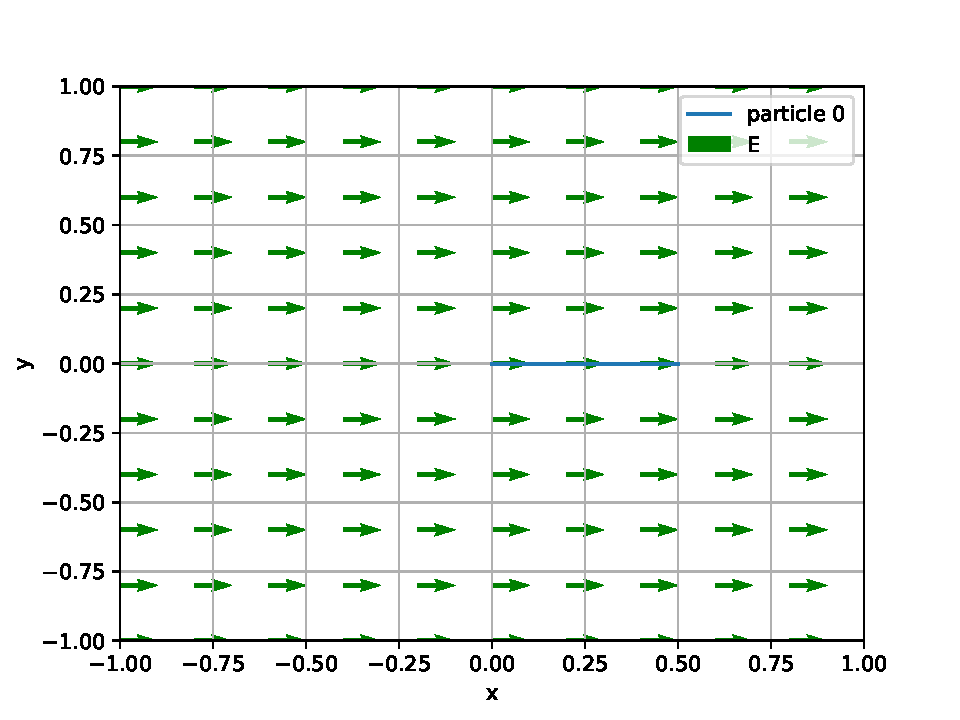
\includegraphics[width=\linewidth]{ex0.pdf}
\caption{Constant electric field.}
\label{fig:ex0}
\end{figure}

The second case is the same particle, starting at position $(0,1,0)$ with velocity $\vec{v}=\hat{x}$ distance units per time subject to a magnetic field $\vec{B}=\vec{z}$, in this case we know (\cite{griff} chapter 5.1.2) the particle will perform a cyclical motion relation $q v_o B= m v_{o}^2/r$ between the orbital velocity and the radius so if I let the simulation run for  $6.28\approx 2 \pi$ time units we expect to see a full circle in the XY plane with radius $r= m v/Bq = 1$, and as see non figure \ref{fig:ex1} this is almost what we see, here I have run the simulation $62.8$ time units for roughly 10 full circles with a total of 10000 time steps, and as is evident the radius has slowly increased, increasing to 1000000 steps seems to solve the problem, but this highlights how unreliable this method is.

\begin{figure}
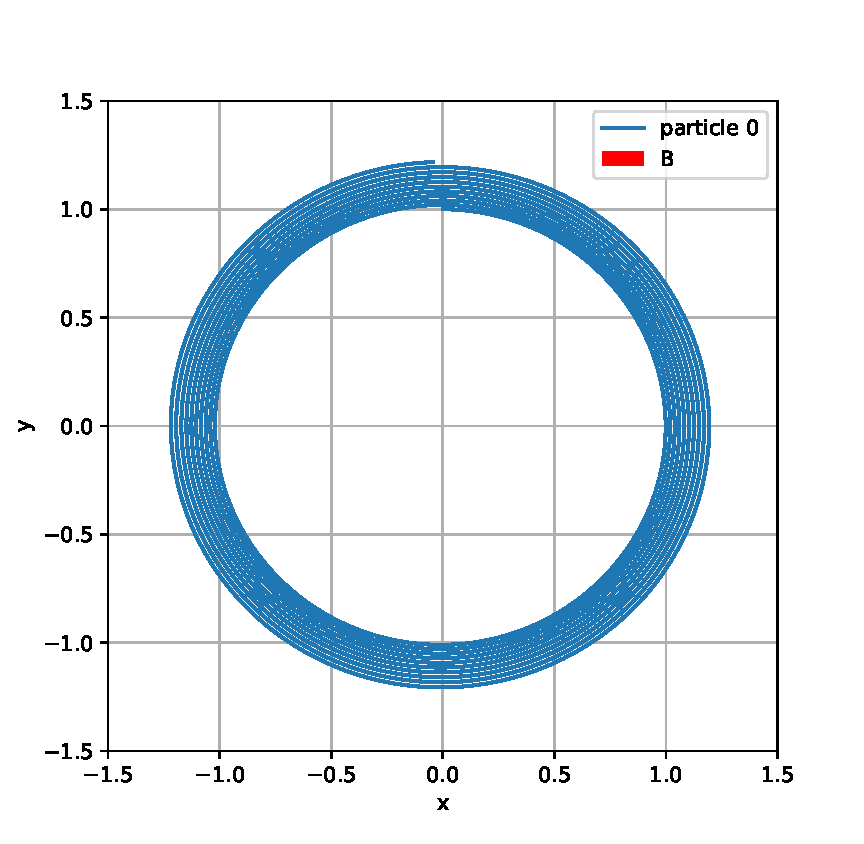
\includegraphics[width=0.5\linewidth]{ex1.pdf}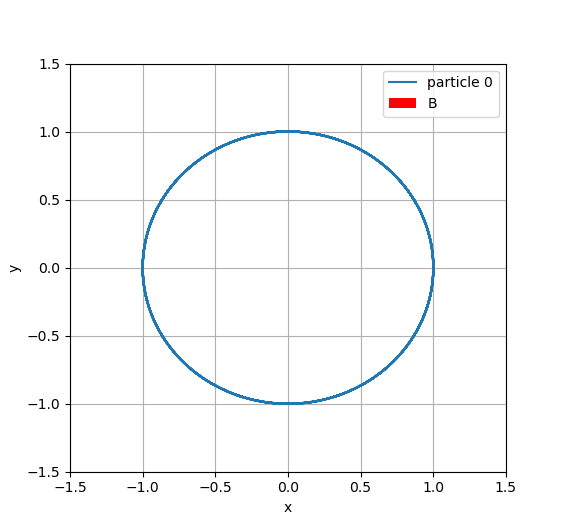
\includegraphics[width=0.5\linewidth]{ex1_1.png}
\caption{Constant magnetic field in Z direction, around 10 full cycles with too low precision (left) and higher precision (right) the high resolution example has been saved as a png, since the vector based pdf version had too large file size.}
\label{fig:ex1}
\end{figure}

The final example is the same particle, starting at rest at $(0,6,0)$ in a electric field $\vec{E}=\hat{x}$ and  $\vec{B}=\hat{z}$. The result on figure \ref{fig:ex2} is Cycloid motion, this was discussed for instance in our electrodynamics course, and this shows that the simulation can handle both fields at once.

\begin{figure}
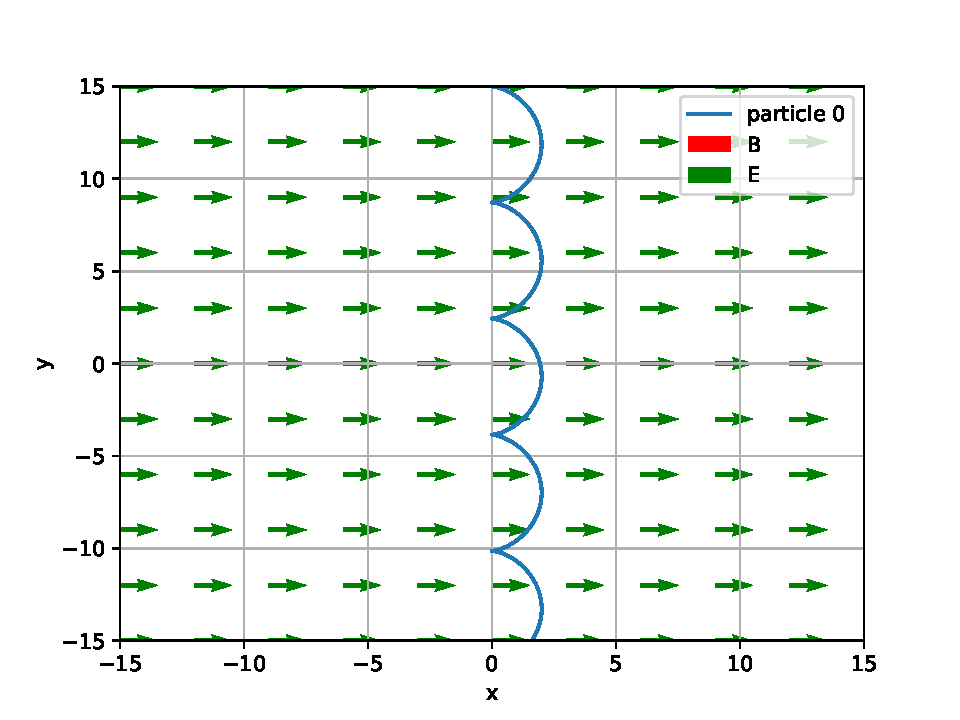
\includegraphics[width=0.5\linewidth]{ex2.pdf}
\caption{Cycloid motion resulting from a combined constant electric and magnetic field.}
\label{fig:ex2}
\end{figure}

\printbibliography

\end{document}

